Our goals in the development of ORES and the deployment of models is to keep the process -- the flow of data from random samples to model training and evaluation open for review, critique, and iteration.  In this section, we'll describe how we implemented transparent replay-ability in our model development process and how ORES outputs a wealth of useful and nuanced information for users.  By making this detailed information available to users and developers, we hope to enable flexibility and power in the evaluation and use of ORES predictions for novel purposes.

\subsection{Collaboratively labeled data}
There are two primary strategies for gathering labeled data for ORES' models: found traces and manual labels.

\leadin{Found traces.} For many models, there are already a rich set of digital traces that can be assumed to reflect a useful human judgement.  For example, in Wikipedia, it's very common that damaging edits will be reverted and that good edits will not be reverted.  Thus the revert action (and remaining traces) can be used to assume that the reverted edit is damaging.  We have developed a re-usable script\footnote{see \emph{autolabel} in \url{https://github.com/wiki-ai/editquality}} that when given a sample of edits, will label the edits as ``reverted\_for\_damage'' or not based on a set of constraints: edit was reverted within 48 hours, the reverting editor was not the same person, and the edit was not restored by another editor.

However, this ``reverted\_for\_damage'' label is problematic in that many edits are reverted not because they are damaging but because they are involved in some content dispute.  Also, the label does not differentiate damage that is a good-faith mistake from damage that is intentional vandalism.  So in the case of damage prediction models, we'll only make use of the ``reverted\_for\_damage'' label when manually labeled data is not available.

Another case of found traces is article quality assessments -- named "wp10" after the Wikipedia 1.0 assessment process originated the article quality assessment scale\footnote{\url{http://enwp.org/WP:WP10}}.  We follow the process developed by Warncke-Wang et al.\cite{wang2017english} to extract the revision of an article that was current at the time of an assessment.  Many other wikis employ a similar process of article quality labeling (e.g. French Wikipedia and Russian Wikipedia), so we can use the same script to extract their assessments with some localization\footnote{see \emph{extract\_labelings} in \url{https://github.com/wiki-ai/articlequality}}.  However other wikis either do not apply the same labeling scheme consistently or at all and manual labeling is our only option.

\begin{figure}[h]
  \centering
  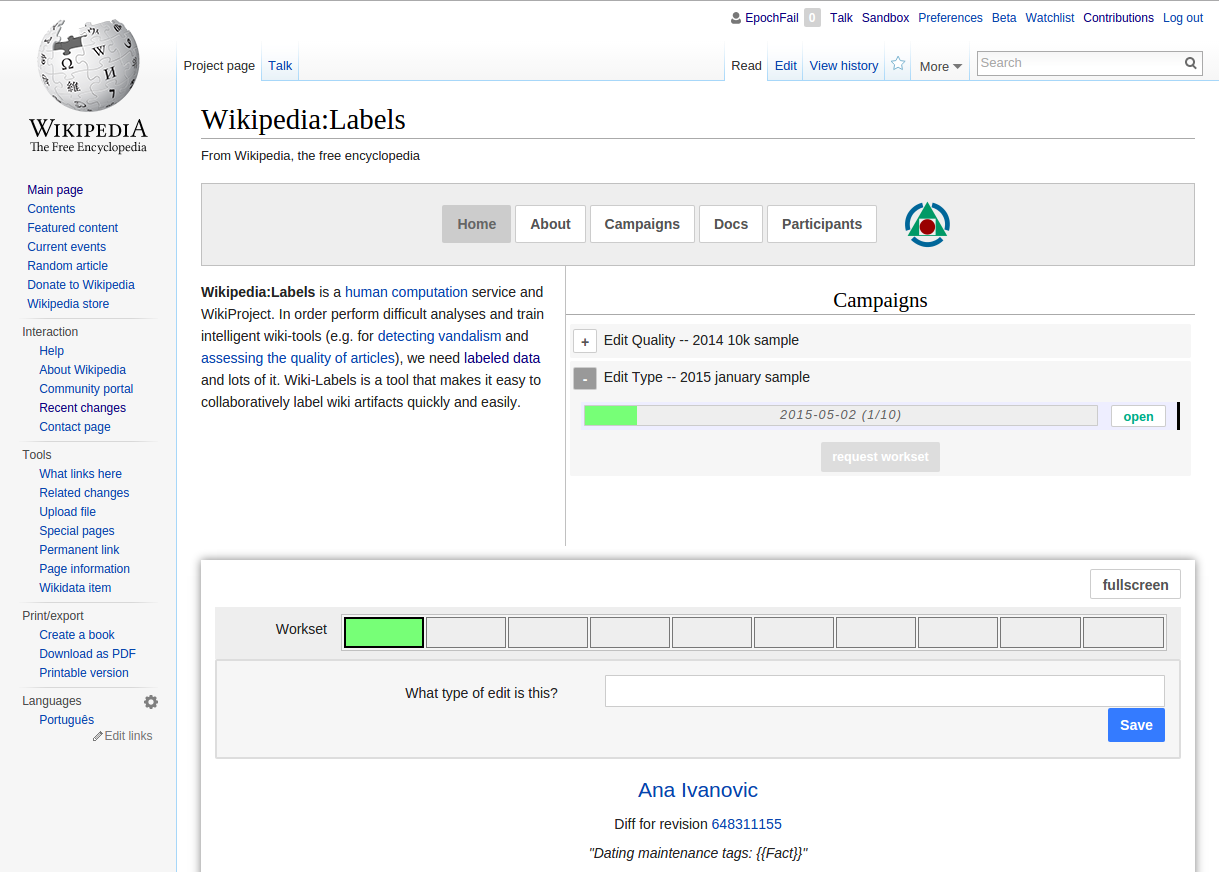
\includegraphics[width=.50\textwidth]{figures/Wiki_labels_gadget}
  \caption{The Wiki labels interface embedded in Wikipedia}
  \label{fig:wikilabels_screenshot}
\end{figure}

\leadin{Manual labeling.}
We hold manual labels for the purposes of training a model to replicate a specific human judgement as a gold standard.  This contrasts with found data that is much easier to come by when it is available.  Manual labeling is expensive upfront from a human labor hours perspective.  In order to minimize the investment of time among our collaborators (mostly volunteer Wikipedians), we've developed a system called "Wiki labels"\footnote{\url{http://enwp.org/:m:Wiki labels}}.  Wiki labels allows Wikipedians to submit judgments of specific samples of Wiki content using a convenient interface and logging in via their Wikipedia account.

To supplement our models of edit quality, we replace the models based on found ``reverted\_for\_damage'' traces with manual judgments where we specifically ask labelers to distinguish ``damaging''/good from ``good-faith''/vandalism.  Using these labels we can build two separate models of that can allow users to filter for edits that are likely to be good-faith mistakes\cite{halfaker2017automated}, to just focus on vandalism, or to focus on all damaging edits broadly.

We've managed to complete manual labeling campaigns article quality for Turkish and Arabic Wikipedia (wp10) as well as item quality in Wikidata.  We've found that, when working with manually labeled data, we can attain relatively high levels of fitness with 150 observations per quality class.

\subsection{Explicit pipelines}
One of our openness goals with regards to how prediction models are trained and deployed in ORES involves making the whole data flow process clear.  Consider the following code that represents a common pattern from our model-building Makefiles:
\begin{figure}[htbp]
        \makebox{\hrulefill}{
        \small
        \begin{verbatim}
datasets/enwiki.human_labeled_revisions.20k_2015.json:
        ./utility fetch_labels \
                https://labels.wmflabs.org/campaigns/enwiki/4/ > $@

datasets/enwiki.labeled_revisions.w_cache.20k_2015.json: \
                datasets/enwiki.labeled_revisions.20k_2015.json
        cat $< | \
        revscoring extract \
                editquality.feature_lists.enwiki.damaging \
                --host https://en.wikipedia.org \
                --extractor $(max_extractors) \
                --verbose > $@

models/enwiki.damaging.gradient_boosting.model: \
                datasets/enwiki.labeled_revisions.w_cache.20k_2015.json
        cat $^ | \
        revscoring cv_train \
                revscoring.scoring.models.GradientBoosting \
                editquality.feature_lists.enwiki.damaging \
                damaging \
                --version=$(damaging_major_minor).0 \
                (... model parameters ...)
                --center --scale > $@
        \end{verbatim}
        \hrule
        \normalsize}
        \caption{Makefile rules for English damage detection model.}
        \label{fig:english_damaging_makefile}
\end{figure}


Essentially, this code helps someone determine where the labeled data comes from (manually labeled via the Wiki Labels system).  It makes it clear how features are extracted (using the utility \texttt{revscoring extract} and the \texttt{enwiki.damaging} feature set).  Finally, this dataset with extracted features is used to cross-validate and train a model predicting the ``damaging'' label and a serialized version of that model is written to a file.  A user could clone this repository, install the set of requirements, and run \texttt{make enwiki\_models} and expect that all of the data-pipeline would be reproduced.

By explicitly using public resources and releasing our utilities and Makefile source code under an open license (MIT), we have essential implemented a turn-key process for replicating our model building and evaluation pipeline.  A developer can review this pipeline for issues knowing that they are not missing a step of the process because all steps are captured in the Makefile.  They can also build on the process (e.g. add new features) incrementally and restart the pipeline.  In our own experience, this explicit pipeline is extremely useful for identifying the origin of our own model building bugs and for making incremental improvements to ORES' models.

At the very base of our Makefile, a user can run \texttt{make models} to rebuild all of the models of a certain type.  We regularly perform this process ourselves to ensure that the Makefile is an accurate representation of the data flow pipeline.  Performing complete rebuild is essential when a breaking change is made to one of our libraries.  The resulting serialized models are saved to the source code repository so that a developer can review the history of any specific model and even experiment with generating scores using old model versions.

\subsection{Model information}
In order to use a model effectively in practice, a user needs to know what to expect from model performance.  E.g. how often is it that when an edit is predicted to be ``damaging'' it actually is? (\emph{precision}) or what proportion of damaging edits should I expect will be caught by the model? (\emph{recall})  The target metric of an operational concern depends strongly on the intended use of the model.  Given that our goal with ORES is to allow people to experiment with the use and reflection of prediction models in novel ways, we sought to build an general model information strategy.

\begin{figure}[htbp]
        \makebox{\hrulefill}{
        \small
        \begin{verbatim}
      "damaging": {
        "type": "GradientBoosting",
        "version": "0.4.0",
        "environment": {"machine": "x86_64", ...},
        "params": {center": true, "init": null, "label_weights": {"true": 10},
                   "labels": [true, false], "learning_rate": 0.01, "min_samples_leaf": 1,
                   ...},
        "statistics": {
          "counts": {"labels": {"false": 18702, "true": 743},
                     "n": 19445,
                     "predictions": {"false": {"false": 17989, "true": 713},
                                     "true": {"false": 331, "true": 412}}},
          "precision": {"labels": {"false": 0.984, "true": 0.34},
                        "macro": 0.662, "micro": 0.962},
          "recall": {"labels": {"false": 0.962, "true": 0.555},
                     "macro": 0.758, "micro": 0.948},
          "pr_auc": {"labels": {"false": 0.997, "true": 0.445},
                     "macro": 0.721, "micro": 0.978},
          "roc_auc": {"labels": {"false": 0.923, "true": 0.923},
                      "macro": 0.923, "micro": 0.923},
          ...
        }
      }
        \end{verbatim}
        \hrule
        \normalsize}
        \caption{Result of \url{https://ores.wikimedia.org/v3/scores/enwiki/?model_info&models=damaging}}
        \label{fig:english_damaging_model_info}
\end{figure}


The output captured in Figure~\ref{fig:english_damaging_model_info} shows a heavily trimmed JSON (human- and machine-readable) output of \emph{model\_info} for the ``damaging'' model in English Wikipedia.  Note that many fields have been trimmed in the interest of space with an ellipsis (``...'').  What remains gives a taste of what information is available.  Specifically, there is structured data about what kind of model is being used, how it is parameterized, the computing environment used for training, the size of the train/test set, the basic set of fitness metrics, and a version number so that secondary caches know when to invalidate old scores.  A developer using an ORES model in their tools can use these fitness metrics to make decisions about whether or not a model is appropriate and to report to users what fitness they might expect at a given confidence threshold.

\subsection{Score documents}
The predictions made by through ORES are also, of course, human- and machine-readable.  In general, our classifiers will report a specific prediction along with a set of probability (likelihood) for each class.  Consider article quality (wp10) prediction output in Figure~\ref{fig:english_damaging_model_info}.

\begin{figure}[htbp]
        \makebox{\hrulefill}{
        \small
        \begin{verbatim}
        "wp10": {
          "score": {
            "prediction": "Start",
            "probability": {
              "FA": 0.0032931301528326693, "GA": 0.005852955431273448,
              "B": 0.060623380484537165, "C": 0.01991363271632328,
              "Start": 0.7543301344435299, "Stub": 0.15598676677150375
            }
          }
        }
        \end{verbatim}
        \hrule
        \normalsize}
        \caption{Result of \url{https://ores.wikimedia.org/v3/scores/enwiki/34234210/wp10}}
        \label{fig:english_damaging_model_info}
\end{figure}

A developer making use of a prediction like this may choose to present the raw prediction ``Start'' (one of the lower quality classes) to users or to implement some visualization of the probability distribution across predicted classed (75\% Start, 16\% Stub, etc.).  They might even choose to build an aggregate metric that weights the quality classes by their prediction weight (e.g. Ross's student support interface\cite{ross2016visualizing} or the \emph{weighted sum} metric from \cite{halfaker2017interpolating}).

\subsection{Threshold optimization}
When we first started developing ORES, we realized that interpreting the likelihood estimates of our prediction models would be crucial to using the predictions effectively.  Essentially, the operational concerns of Wikipedia's curators need to be translated into a likelihood threshold.  For example, counter-vandalism patrollers seek catch all (or almost all) vandalism before it is allowed to stick in Wikipedia for very long.  That means they have an operational concern around the \emph{recall} of a damage prediction model.  They'd also like to review as few edits as possible in order to catch that vandalism.  So they have an operational concern around the \emph{filter rate} -- the proportion of edits that are not flagged for review by the model\cite{halfaker2016notes}.

By finding the threshold of prediction likelihood that optimizes the filter-rate at a high level of recall, we can provide vandal-fighters with an effective trade-off for supporting their work.  We refer to these optimizations in ORES as \emph{threshold optimizations} and ORES provides information about these thresholds in a machine-readable format so that tools can automatically detect the relevant thresholds for their wiki/model context.

Originally, when we developed ORES, we defined these threshold optimizations in our deployment configuration.  But eventually, it became apparent that our users wanted to be able to search through fitness metrics to adapt their own optimizations.  Adding new optimizations and redeploying quickly became a burden on us and a delay for our users.  So we developed a syntax for requesting an optimization from ORES in realtime using fitness statistics from the models tests. E.g. \texttt{maximum recall @ precision >= 0.9} gets a useful threshold for a counter-vandalism bot or \texttt{maximum filter\_rate @ recall >= 0.75} gets a useful threshold for semi-automated edit review (with human judgement).

\begin{figure}[htbp]
        \makebox{\hrulefill}{
        \small
        \begin{verbatim}
  {"threshold": 0.299, ...,
   "filter_rate": 0.88, "fpr": 0.097, "match_rate": 0.12,
   "precision": 0.215, "recall": 0.751}
        \end{verbatim}
        \hrule
        \normalsize}
        \caption{Result of \url{https://ores.wikimedia.org/v3/scores/enwiki/?models=damaging&model_info=statistics.thresholds.true.'maximum filter_rate @ recall >= 0.75'}}
        \label{fig:english_damaging_threshold_optimization}
\end{figure}

This result shows that, when a threshold is set on 0.299 likelihood of damaging=true, then you can expect to get a recall of 0.751, precision of 0.215, and a filter-rate of 0.88.  While the precision is low, this threshold reduces the overall workload of vandal-fighters by 88\% while still catching 75\% of (the most egregious) damaging edits.

\subsection{Dependency injection and interrogability}
From a technical perspective, ORES is a algorithmic "scorer" container system.  It's primarily designed for hosting machine classifiers, but it is suited to other scoring paradigms as well.  E.g. at one point, our experimental installation of ORES hosted a Flesch-Kincaid readability scorer.  The only real constraints are that the scorer must express it's inputs in terms of "dependencies" that ORES knows how to solve and the scores must be presentable in JSON (Javascript Object Notation).

\subsubsection{Dependency injection}
One of the key features of ORES that allows scores to be generated in an efficient and flexible way is a dependency injection framework.

\leadin{Efficiency.}
For example, there are several features that go into the "damaging" prediction model that are drawn from the \emph{diff} of two versions of an articles text (words added, words removed, badwords added, etc.)  Because all of these features ``depend'' on the \emph{diff}, the dependency solver can make sure that only one \emph{diff} is generated and that all subsequent features make use of that shared data.

ORES can serve multiple scores in the same request.  E.g. a user might want to gather a set of scores: "edit type", "damaging", and "good-faith".  Again, all of these prediction models depend on features related to the edit \emph{diff}.  ORES can safely combine all of the features required for each of the requested models and extract them with their shared dependencies together.  Given that feature extraction tends to take the majority of time in a real-time request request (partially for fetching data [IO], partially for computation time [CPU]), this allows the scoring for multiple, similar models to take roughly the same amount of time as scoring a single model.

\leadin{Flexibility.} When developing a model, it's common to experiment with different feature sets.  A natural progression in the life of a model in the wild involves the slow addition of new features that prove useful during experimentation.  By implementing a dependency system and a dependency solver, a model can communicate to ORES which features it needs and ORES can provide those features.  At no point does a model developer need to teach ORES how to gather new data.  All of the information needed for the solver to solve any given feature set is wrapped up in the dependencies.

\subsubsection{Interrogability}
The flexibility provided by the dependency injection framework let us implement a novel strategy for exploring \emph{how} ORES' models make predictions.  By exposing the features extracted to ORES users and allowing them to inject their own features, we can allow users to ask how predictions would change if the world were different.  Let's look at an example to demonstrate.  Let's say you wanted to explore how ORES judges unregistered (anon) editors differently from registered editors.


\begin{figure}[htbp]
        \makebox{\hrulefill}{
        \small
        \begin{verbatim}
        "damaging": {
          "features": {
            ...
            "feature.revision.user.is_anon": false,
            ...
          },
          "score": {
            "prediction": false,
            "probability": {
              "false": 0.938910157824447,
              "true": 0.06108984217555305
            }
          }
        }
        \end{verbatim}
        \hrule
        \normalsize}
        \caption{Result of \url{https://ores.wikimedia.org/v3/scores/enwiki/34234210/damaging?features}}
        \label{fig:english_damaging_features}
\end{figure}

This essentially means that the "damaging" prediction model concludes that the edit identified by the \emph{revision ID} of 34234210 is not damaging with 93.9\% confidence.  We can ask ORES to make a prediction about the exact same edit, but to assume that the editor was unregistered.

\begin{figure}[htbp]
        \makebox{\hrulefill}{
        \small
        \begin{verbatim}
        "damaging": {
          "features": {
            ...
            "feature.revision.user.is_anon": true,
            ...
          },
          "score": {
            "prediction": false,
            "probability": {
              "false": 0.9124151990561908,
              "true": 0.0875848009438092
            }
          }
        }
        \end{verbatim}
        \hrule
        \normalsize}
        \caption{Result of \url{https://ores.wikimedia.org/v3/scores/enwiki/34234210/damaging?features&feature.revision.user.is_anon=true}}
        \label{fig:english_damaging_features}
\end{figure}

If this edit were saved by an anonymous editor, ORES would still conclude that the edit was not damaging, but with less confidence (91.2\%).  By following a pattern like this for a single edit or a set of edits, we can get to know how ORES prediction models account for anonymity.

This is a very powerful tool for interrogating ORES.  Imagine being able to ask a law enforcement officer if they feel like they have probable cause for a search and then asking again how their answer would change if the suspect were black.

Interrogability isn't only useful for checking to see where ORES biases originate and what effects they have on predictions.  For example, Ross has started using our article quality prediction models (\emph{wp10}) as a method for suggesting work to new editors\footnote{\url{https://dashboard-testing.wikiedu.org}}.  By asking ORES to score a student's draft and then asking ORES to reconsider the predicted quality level of the article with \emph{one more header}, \emph{one more image} , or \emph{one more citation}, they've built an intelligent user interface that can automatically recommend the most productive development to the article -- the change that will most likely bring it to a higher quality level.
